\chapter{Estudio sobre el acero F138}\label{C:F138}
\graphicspath{{./figs/04_F138/}}

En este capítulo se estudia la microestructura del acero inoxidable F138.
Este acero es de tipo austenítico, es decir que tiene una estructura FCC y tiene una composición que puede verse en la Tabla \ref{tab:F138Comp}.
Se caracteriza por tener una elevada resistencia a la corrosión, lo que lo hace útil para aplicaciones biomédicas y en energía nuclear.
Según el estudio realizado por Scheriau et al \cite{Scheriau2011} la deformación plástica severa se caracteriza por dos modos de deformación principales maclado mecánico (con maclas de 10-20 nm de ancho) y bandas de corte submicrométricas que dividen el material en bloques micrométricos de láminas de maclas.
Liu et al. \cite{Liu2010} observaron una respuesta similar en un acero 316L sometido a deformación plástica dinámica, donde la estructura final evolucionó hacia una configuración de granos micrométricos de austenita junto con maclas nanométricas, confiriéndole al material una tensión de fluencia casi cinco veces mayor que aquella correspondiente a la estructura inicial de granos grandes.

\begin{table}[!htb]
\centering
\caption{Composición del acero inoxidable F138 (\% en peso dado por el fabricante)}
\label{tab:F138Comp}
\begin{tabular}{|c|c|c|c|c|c|c|c|c|c|c|}
\hline
\rowcolor[HTML]{BBDAFF} 
\textbf{Fe} & \textbf{Cr} & \textbf{Ni} & \textbf{Mo} & \textbf{Mn} & \textbf{Si} & \textbf{Cu} & \textbf{N} & \textbf{C} & \textbf{P} & \textbf{S} \\ \hline
          &    17.33  &   14.31   &   2.79    &   1.79    &  0.30     &   0.09    &   0.079   &  0.015    &   0.022   &   0.002   \\ \hline
\end{tabular}
\end{table}

El 2.5\% de Mo agregado mejora la resistencia a la corrosión, y al encontrarse en solución sólida contribuye a reducir la movilidad de las dislocaciones \cite{Chowdhury2005}.

El grupo de trabajo al que pertenece el autor de esta tesis tiene antecedentes de trabajo, tanto en muestras laminadas como en muestras deformadas por medio de la técnica de \textit{Deformación de Igual Canal Angular} (ECAE, por sus siglas en inglés)\cite{Devincentis2015PhD,Devincentis2017}, aunque los estudios realizados se concentraron previamente en mediciones de EBSD y en estudios de ancho de pico a través de los métodos de Williamson-Hall y CMWP.
En la Sec. \ref{S:F138Nati} se realiza un repaso de los principales resultados que se tienen sobre este material, mientras que en la Sec. \ref{S:F138LANG} se aplica el método de Langford a muestras de acero F138 laminadas hasta lograr una reducción de la reducción transversal del 70\,\%.

\nomenclature{ECAE}{Equal Angle Angular Extrusion, Deformación de Igual Canal Angular}
\section{Estado del arte en el estudio de la microestructura}\label{S:F138Nati}
En la Fig. \ref{fig:F138PF} se encuentran las FP recalculadas a partir de las mediciones de textura realizadas en sincrotrón, donde pueden apreciarse la presencia de la fibra {110}\textless uvw\textgreater.
Si se observa la FDO de la Fig. \ref{fig:F138ODF} puede apreciarse que la fibra tiene mayor intensidad en la componente Goss (\{110\}\textless 001\textgreater) y G/B(T) (\{110\}\textless 111\textgreater).
La primera es de esperarse en materiales laminados (?)[ref], mientras que la segunda se asocia a la baja energía de falla de apilamiento en aceros\cite{Sathiaraj2015,Saleh2012}.

\begin{figure}[!htb]
  \centering
  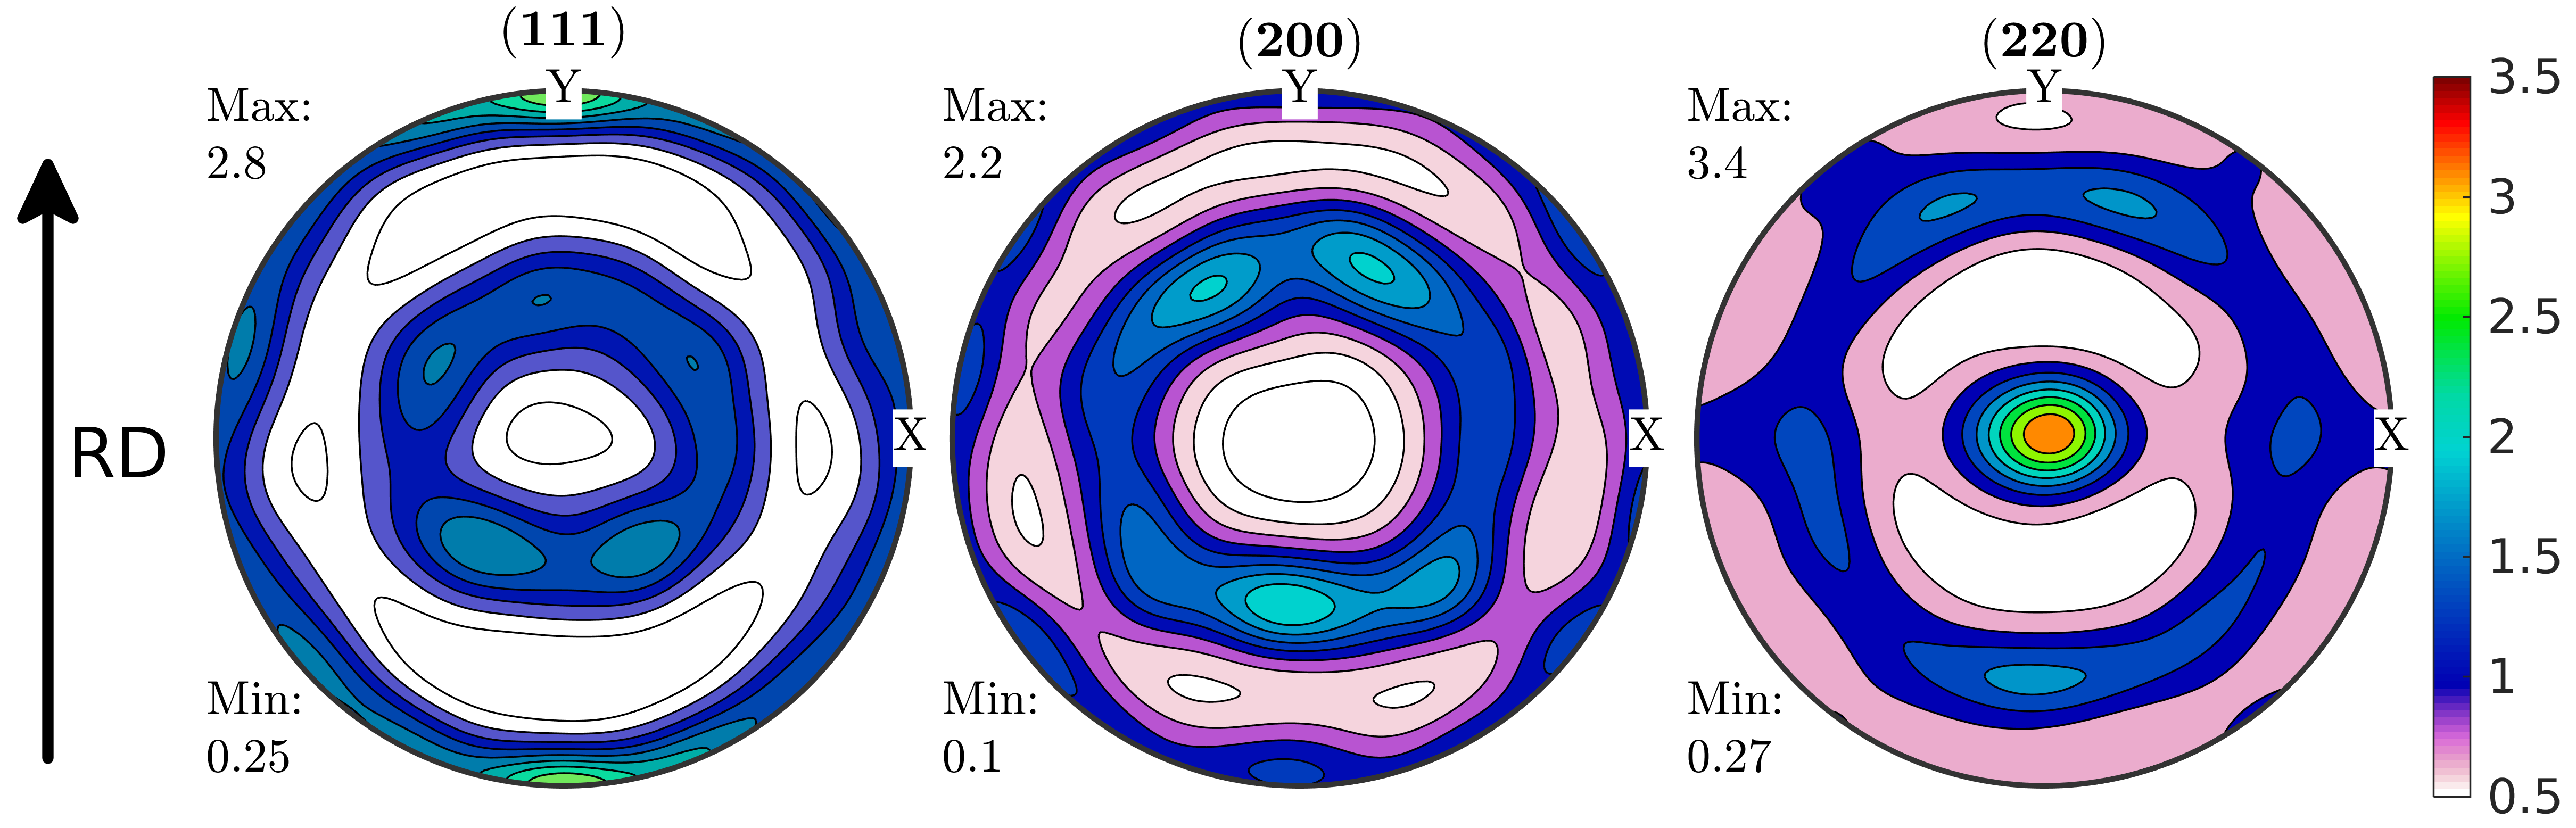
\includegraphics[width=\textwidth]{F138_Rec_RD}
  \caption{Textura F138 con sincrotron}
  \label{fig:F138PF}
\end{figure}


\begin{figure}[!htb]
  \centering
  \includegraphics[width=\textwidth]{F138_odf}
  \caption{ODF del F138}
  \label{fig:F138ODF}
\end{figure}


\newpage
\section{Estudio de la microestructura por el método de Langford y figuras de polos generalizadas}\label{S:F138LANG}
Al observar las FDO Generalizadas de Tamaño de cristalita y deformación, Figs. \ref{fig:F138Size} y \ref{fig:F138Strain} respectivamente, puede verse un comportamiento similiar al observado en el acero libre de intersticiales (Cap. \ref{C:IF}) en donde ciertas componentes favorecidas por la textura tienen mayor tamaño de cristalita y acumulan menos deformación, lo que en este caso se traduce a una menor densidad de dislocaciones.
En este caso puede verse que es la componente Goss es la componente que ``más limpia'', mientras que en la componente G/B(T) se tienen dominios un poco más grandes, pero con menor cantidad de dislocaciones acumuladas.
\begin{figure}[!htb]
  \centering
  \includegraphics[width=\textwidth]{F138_size_odf}
  \caption{Size ODF F138}
  \label{fig:F138Size}
\end{figure}

\begin{figure}[!htb]
  \centering
  \includegraphics[width=\textwidth]{F138_strain_odf}
  \caption{Strain ODF}
  \label{fig:F138Strain}
\end{figure}




\newpage
\section{Discusión de resultados}\label{S:F138Dis}
\newpage
\section{Conclusiones}\label{S:F138Conclusiones}
